% Chapter Template

\chapter{Results} % Main chapter title
\label{chap:results} % Change X to a consecutive number; for referencing this chapter elsewhere, use \ref{ChapterX}
This chapter will summarize the results of this work. First, the results of simulating the susceptible population
in the region of Hesse will be presented. Then the results of a sensitivity analysis for the variables $\alpha$ and
$q$ will be shown. Specifically the sensitivity analysis will later be used in \hyperref[chap:discussion]{Chapter
\ref*{chap:discussion} - Discussion} to explain the results of the simulations.


%----------------------------------------------------------------------------------------
%	SECTION 1
%----------------------------------------------------------------------------------------

\section{Simulating the susceptible population of Hesse}
\textcolor{red}{check your tenses and make sure they make sense!}
\textcolor{red}{remove data point/day inconsistencies}

During this work we simulated the susceptible population of Hesse. 26 regions were simulated over a time period of
76, 60 and 50 days respectively. We will present both the absolute and percentage difference between the simulated
and the original data for each time frame.

\textcolor{red}{redo box plots with x-axis description}

%-----------------------------------
%	SUBSECTION 1
%-----------------------------------
\subsection{Simulating susceptibles in a 76 day time frame}
We first wanted to observe how well the simulation performs in a time frame of 76 days. Since the number of susceptible
individuals is much greater then any other group at any given data point, changes in this group can be difficult to
observe. Because of this we decided to calculate and compare the number of individuals that migrated from the susceptible
to the exposed group instead. This was done by subtracting the number of susceptible individuals at data point \I{t=x} from
the start point \I{t=0}. The result is the total change of susceptibles at any given time point, which is equivalent to the 
sum of all exposed individuals at any given time point. These results are much easier to compare and understand.
\hyperref[fig:76_sim_expl]{figure \ref*{fig:76_sim_expl}} shows three graphs that illustrate this process.


\begin{figure}
	\centering
	\begin{subfigure}[b]{0.3\textwidth}
		\centering
		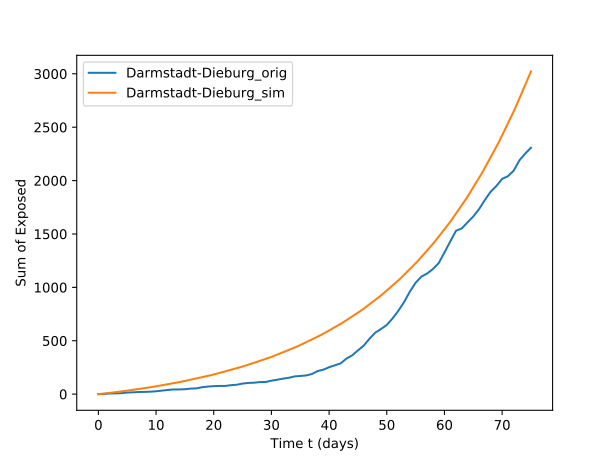
\includegraphics[width=\textwidth]{./figures/76d/24_Darmstadt-Dieburg.png}	
		\caption{}
	\end{subfigure}
	\hfill
	\begin{subfigure}[b]{0.3\textwidth}
		\centering
		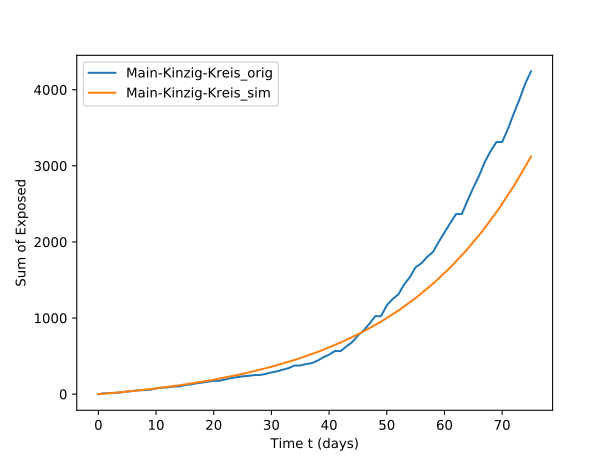
\includegraphics[width=\textwidth]{./figures/76d/13_Main-Kinzig-Kreis.png}	
		\caption{}
	\end{subfigure}
	\hfill
	\begin{subfigure}[b]{0.3\textwidth}
		\centering
		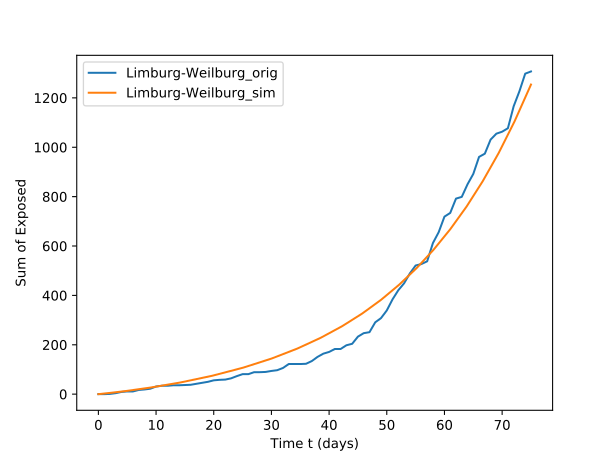
\includegraphics[width=\textwidth]{./figures/76d/10_Limburg-Weilburg.png}	
		\caption{}
	\end{subfigure}
	\caption{Three exemplary results of a simulation of the exposed individuals.
		The original (``orig'') data is drawn in blue and the simulated (``sim'') data is drawn in orange.
		The number of simulated exposed individuals can be greater (image (A), region ``Darmstadt Dieburg''), smaller 
		(image (B), region ``Mein Kinzig Kreis'') or about the same (image (C), region ``Limburg Weilburg''), as 
		the originally observed number of exposed.
		}
	\label{fig:76_sim_expl}
\end{figure}

Furthermore we analyzed the percentage deviation of original and simulated data for each time step in each region. The results
are shown in a box plot in \hyperref[fig:76_sim_box]{figure \ref*{fig:76_sim_box}}. The three regions ``Werra-Meissner-Kreis'',
``Marburg-Biedenkopf'' and ``Limburg-Weilburg'' are listed separately in figure \ref*{fig:76_sim_box}, in order to make the scales
more readable.


\begin{figure}
	\centering
	\begin{subfigure}[b]{0.4\textwidth}
		\centering
		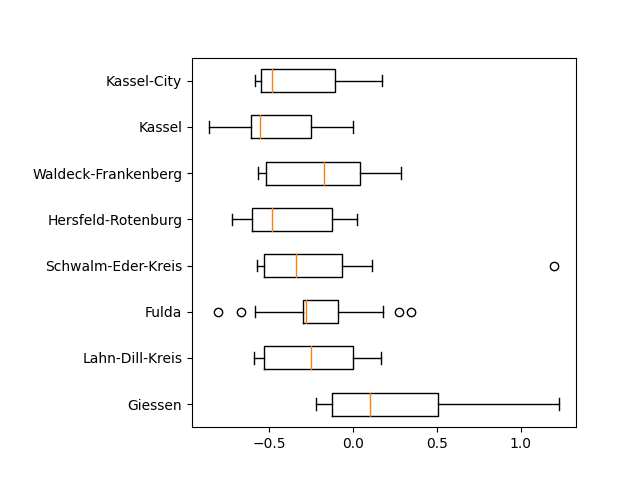
\includegraphics[width=\textwidth]{./figures/76d/deviation_box76_alt1.png}	
	\end{subfigure}
	\begin{subfigure}[b]{0.4\textwidth}
		\centering
		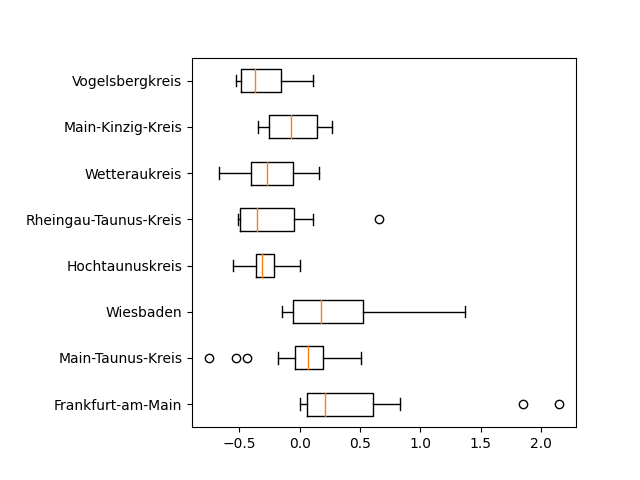
\includegraphics[width=\textwidth]{./figures/76d/deviation_box76_alt2.png}	
	\end{subfigure}
	\begin{subfigure}[b]{0.4\textwidth}
		\centering
		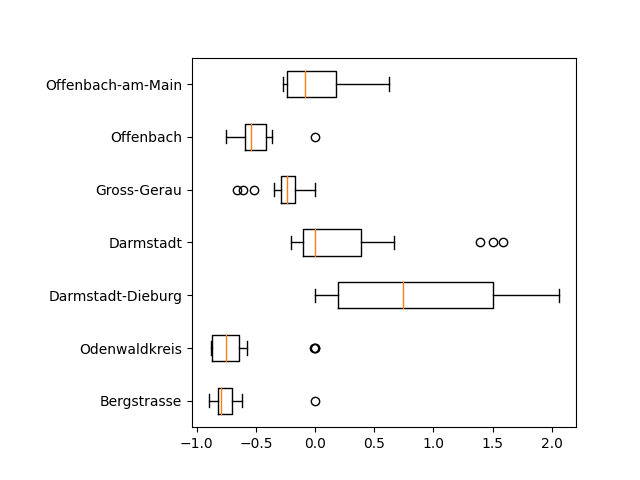
\includegraphics[width=\textwidth]{./figures/76d/deviation_box76_alt3.png}	
	\end{subfigure}
	\begin{subfigure}[b]{0.4\textwidth}
		\centering
		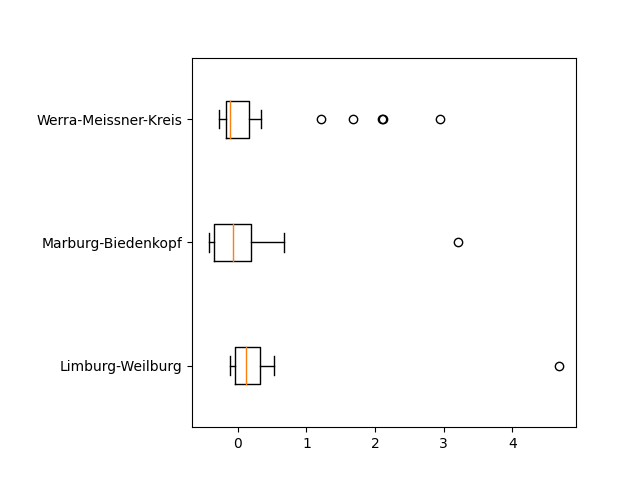
\includegraphics[width=\textwidth]{./figures/76d/deviation_box76_alt4.png}	
	\end{subfigure}
	\caption{Shown are box plots of the percentage deviation, of every simulated region relative to the original data.}
	\label{fig:76_sim_box}
\end{figure}

\textcolor{red}{rephrase for deviation factor and meaning}
Figure \ref*{fig:76_sim_box} shows that the simulated regions have a wide range of median values regarding the deviation.
The numbers are ranging between a median deviation factor of about -0.8 and +0.75. This means, that the model calculated
between 80 percent less or 75 percent more infection events, compared to the original data. Apart from these extreme cases, 12 out of
26 regions have an absolute, median deviation of less then 25 percent, 21 of the 26 regions show an absolute median below 50 percent
and 25 of the 26 regions have a median of less then 75 percent. Only the region ``Berstrasse'' had a higher deviation with
about -79.16 percent. Many of the plots are skewed right (\textcolor{red}{explain and describe better, also add data to Appendix!!!}).



%-----------------------------------
%	SUBSECTION 2
%-----------------------------------
\subsection{Simulating susceptibles in a 60 day time frame}
In order to explore how well the model is working with a smaller data set, the same optimization process as in the previous section was
applied to a 60 day data set. Only the first 60 days of the previously chosen time frame were simulated, the other 16 days were
simply removed. \hyperref[fig:60_sim_expl]{Figure \ref*{fig:60_sim_expl}} shows three exemplary graphs of the simulation results.
For better comparability, the same regions were chosen as in previous section. The results were extrapolated in order to better visualize
the trend of the simulation result.

\begin{figure}
	\centering
	\begin{subfigure}[b]{0.3\textwidth}
		\centering
		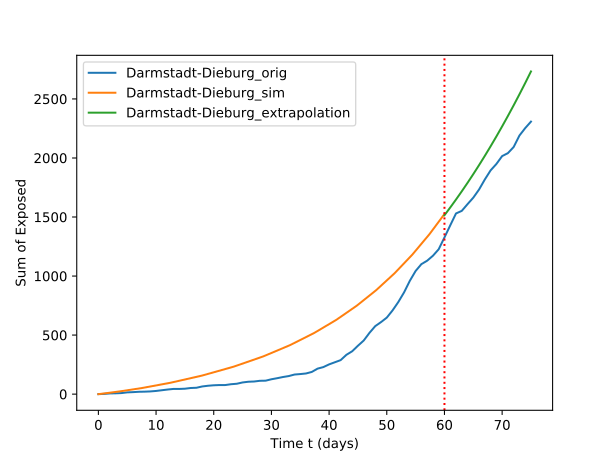
\includegraphics[width=\textwidth]{./figures/60d/24_Darmstadt-Dieburg.png}	
		\caption{}
	\end{subfigure}
	\hfill
	\begin{subfigure}[b]{0.3\textwidth}
		\centering
		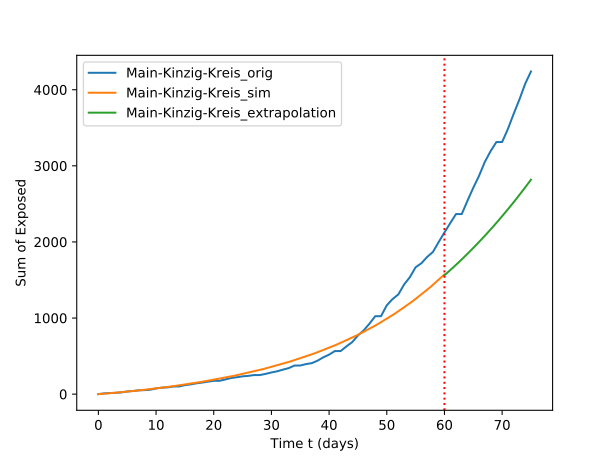
\includegraphics[width=\textwidth]{./figures/60d/13_Main-Kinzig-Kreis.png}	
		\caption{}
	\end{subfigure}
	\hfill
	\begin{subfigure}[b]{0.3\textwidth}
		\centering
		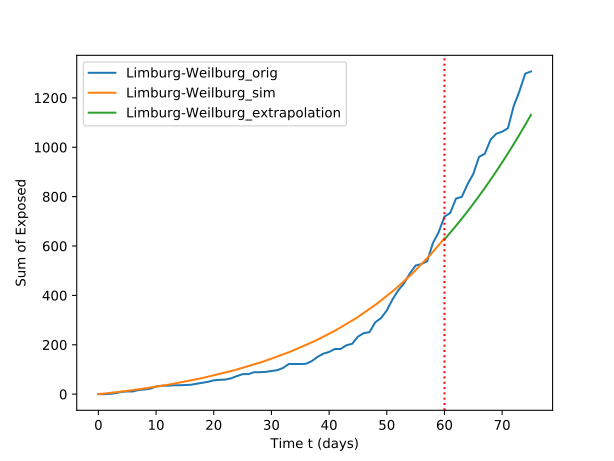
\includegraphics[width=\textwidth]{./figures/60d/10_Limburg-Weilburg.png}	
		\caption{}
	\end{subfigure}
	\caption{Three exemplary results of a simulation of the exposed individuals. The original (``orig'') data is drawn in blue,
		the simulated (``sim'') data is drawn in orange and the extrapolation of the simulated data (``extrapolation'') is
		drawn in green. The vertical red dotted line marks the transition from simulated to extrapolated data.
		}
	\label{fig:60_sim_expl}
\end{figure}

Figure \ref*{fig:60_sim_expl} shows that the general trend of the simulations remains similar to the simulations with 76 data points.
In all three regions, the extrapolated data points show a slightly slower increase in infections compared to the simulations
with 76 days in figure \ref*{fig:76_sim_expl}.

Similar to the previous section, we calculated the deviation of each data point for
each region and expressed the results in a set of box plots. The results are shown in figure \ref*{fig:60_sim_box}. Only data points
that were actually simulated were included into this analysis. Extrapolated data points were not used.

\textcolor{red}{more text for box plots}



\begin{figure}
	\centering
	\begin{subfigure}[b]{0.4\textwidth}
		\centering
		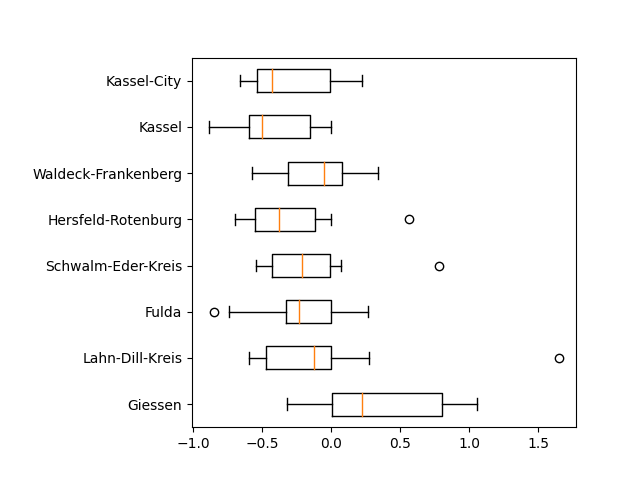
\includegraphics[width=\textwidth]{./figures/60d/deviation_box60_alt1.png}	
	\end{subfigure}
	\begin{subfigure}[b]{0.4\textwidth}
		\centering
		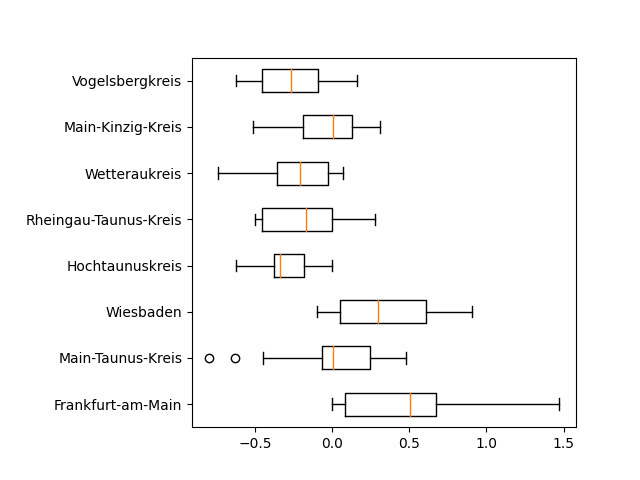
\includegraphics[width=\textwidth]{./figures/60d/deviation_box60_alt2.png}	
	\end{subfigure}
	\begin{subfigure}[b]{0.4\textwidth}
		\centering
		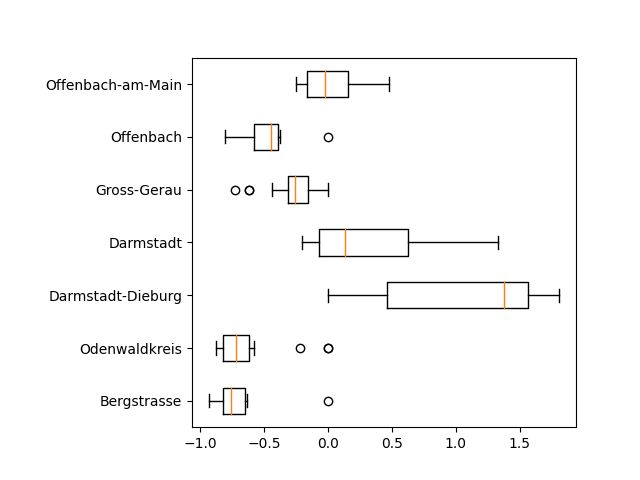
\includegraphics[width=\textwidth]{./figures/60d/deviation_box60_alt3.png}	
	\end{subfigure}
	\begin{subfigure}[b]{0.4\textwidth}
		\centering
		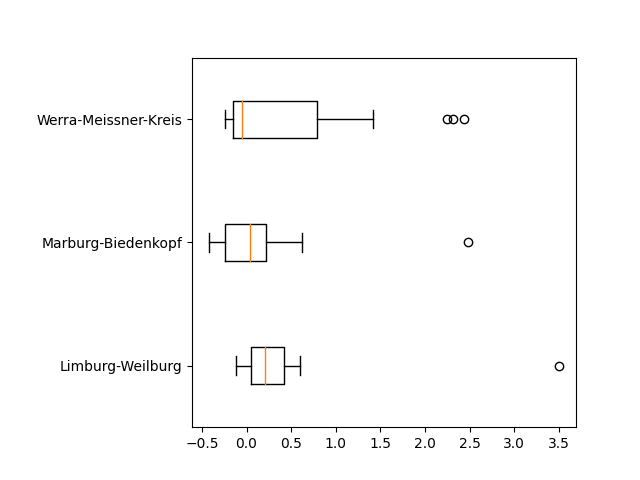
\includegraphics[width=\textwidth]{./figures/60d/deviation_box60_alt4.png}	
	\end{subfigure}
	\caption{Shown are box plots of the percentage deviation, of every simulated region relative to the original data.}
	\label{fig:60_sim_box}
\end{figure}

As with the graphs described before, the deviation results of the 60 data point simulation are largely comparable to the 76
data point deviation results. The maximum and minimum median deviation of all regions is higher compared to previous results,
lying between about -76 percent and 138 percent. However, 14 of the 26 regions displayed an absolute, median deviation of less than
25 percent, two more than in the previous experiment. 21 of 26 regions had an absolute, median deviation of less than 50 percent
and 24 or 26 regions had an absolute, median deviation of less then 75 percent deviation. The two regions with a deviation higher
than 75 percent were ``Bergstrasse'' with -75.52 percent and ``Darmstadt-Dieburg'' with 137.31 percent median deviation. As in
the previous section many box plots are skewed to the right, however this effect seems to be less prominent then in the 76 data
point simulation.


%-----------------------------------
%	SUBSECTION 3
%-----------------------------------
\subsection{Simulating susceptibles in a 50 day time frame}
The last simulation that was performed, was a simulation with 50 data points. As described in the previous section with
60 data points, simulations and optimization steps were performed on a truncated data set, where the last 26 of the total
76 data points were removed. \hyperref[fig:50_sim_expl]{Figure \ref*{fig:50_sim_expl}} shows three exemplary graphs of this
experiment. As previously, the same regions were chosen as for the 76 data point experiment. 
\textcolor{red}{add more explanation and description once graphs are there}

\begin{figure}
	\centering
	\begin{subfigure}[b]{0.3\textwidth}
		\centering
		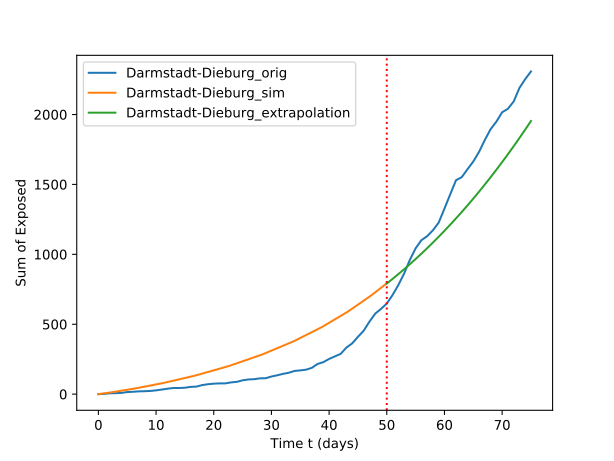
\includegraphics[width=\textwidth]{./figures/50d/24_Darmstadt-Dieburg.png}	
		\caption{}
	\end{subfigure}
	\hfill
	\begin{subfigure}[b]{0.3\textwidth}
		\centering
		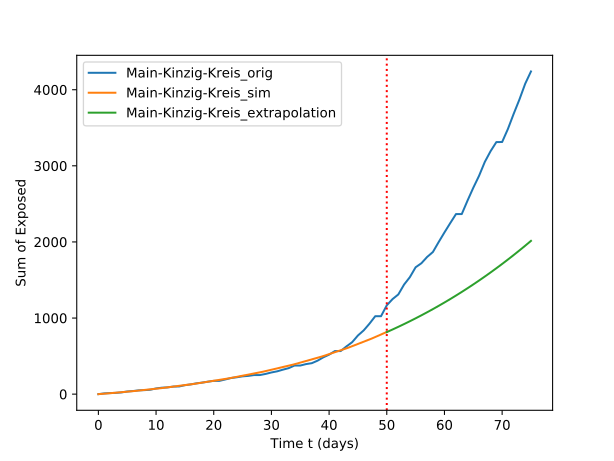
\includegraphics[width=\textwidth]{./figures/50d/13_Main-Kinzig-Kreis.png}	
		\caption{}
	\end{subfigure}
	\hfill
	\begin{subfigure}[b]{0.3\textwidth}
		\centering
		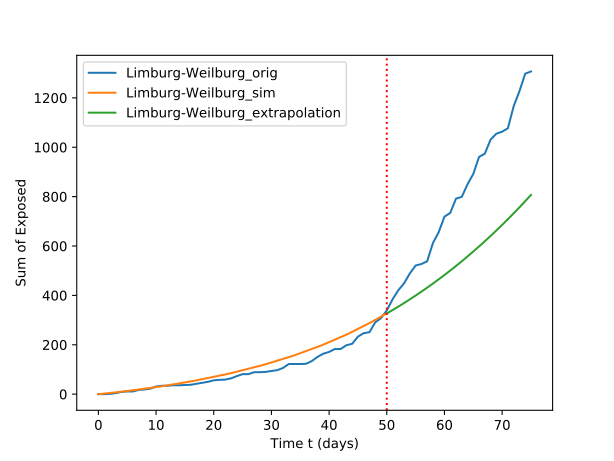
\includegraphics[width=\textwidth]{./figures/50d/10_Limburg-Weilburg.png}	
		\caption{}
	\end{subfigure}
	\caption{Add caption
		}
	\label{fig:50_sim_expl}
\end{figure}
In this experiment, all three
regions show a stronger trend towards a negative deviation, compared to the previous two experiments. While the regions of
the graphs, that were simulated based on the provided data points, looks somewhat similar, the overall trend visualized by
the extrapolation shows a strong deviation.

As with the 60 data point analysis, we also performed the deviation analysis on the 50 data point data set. As previously described
only actually simulated data points were included into the analysis. Extrapolated data points were not used. The results of this
analysis are shown in \hyperref[fig:50_sim_box]{Figure \ref*{fig:50_sim_box}}.

\begin{figure}
	\centering
	\begin{subfigure}[b]{0.4\textwidth}
		\centering
		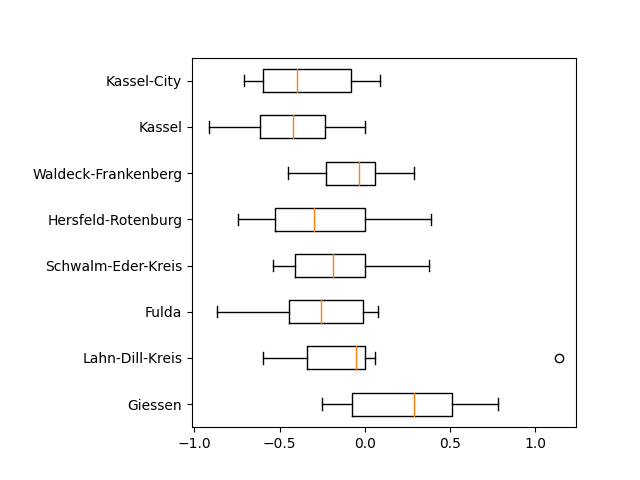
\includegraphics[width=\textwidth]{./figures/50d/deviation_box50_alt1.png}	
	\end{subfigure}
	\begin{subfigure}[b]{0.4\textwidth}
		\centering
		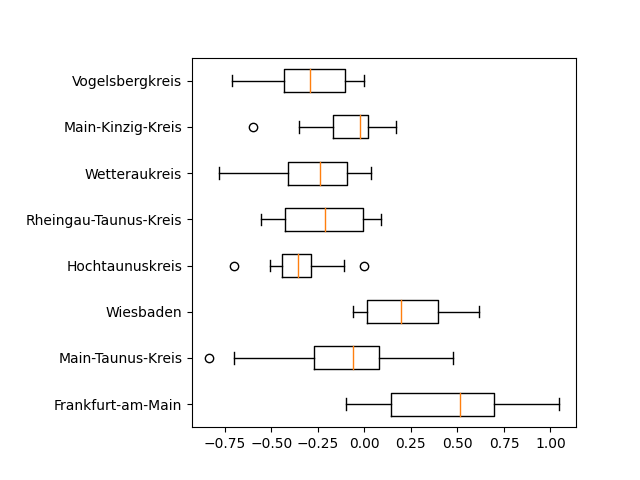
\includegraphics[width=\textwidth]{./figures/50d/deviation_box50_alt2.png}	
	\end{subfigure}
	\begin{subfigure}[b]{0.4\textwidth}
		\centering
		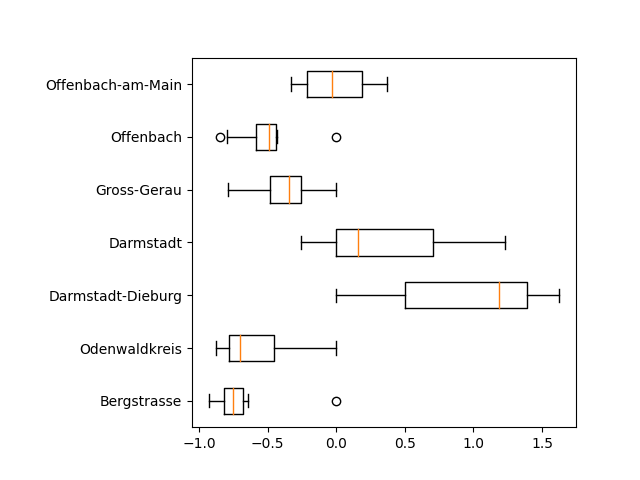
\includegraphics[width=\textwidth]{./figures/50d/deviation_box50_alt3.png}	
	\end{subfigure}
	\begin{subfigure}[b]{0.4\textwidth}
		\centering
		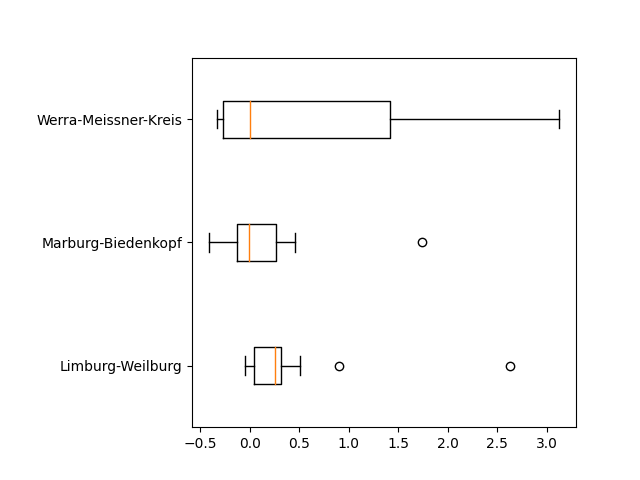
\includegraphics[width=\textwidth]{./figures/50d/deviation_box50_alt4.png}	
	\end{subfigure}
	\caption{Shown are box plots of the percentage deviation, of every simulated region relative to the original data.}
	\label{fig:50_sim_box}
\end{figure}


%----------------------------------------------------------------------------------------
%	SECTION 2
%----------------------------------------------------------------------------------------

\section{Simulation deviation in relation to region population}





%----------------------------------------------------------------------------------------
%	SECTION 3
%----------------------------------------------------------------------------------------

\section{Sensitivity analysis of $\alpha$ and $q$}

